% One-slide talk — Scientific Studio (week 8)
% Compile: xelatex studio/slide_main.tex (from repo root)
\documentclass[landscape,a4paper,11pt]{article}
\usepackage[margin=1.4cm]{geometry}
\usepackage{fontspec}
\usepackage{polyglossia}
\setmainlanguage{russian}
\setotherlanguage{english}
\setmainfont{Times New Roman}
\setsansfont{Helvetica Neue}
\usepackage{amsmath,amssymb}
\usepackage{graphicx}
\usepackage{xcolor}
\usepackage{enumitem}
\setlist{nosep,leftmargin=1.2em}

\definecolor{accent}{RGB}{180,30,40}
\definecolor{msgbg}{RGB}{244,248,244}
\definecolor{msgline}{RGB}{44,160,44}
\pagestyle{empty}

\begin{document}

\begin{center}
{\LARGE\bfseries Однослайдовый доклад: когда окупается планирование в рекомендациях}\\[2pt]
{\color{accent}\rule{\textwidth}{1.2pt}}
\end{center}

\vspace{-4pt}
\noindent\begin{minipage}[t]{0.46\textwidth}
\vspace{0pt}
\textbf{Постановка (MF-MDP).} Состояние $s=(P,u)$, $P=A^{-1}$; оптимистичный переход
(принятие всегда):
\[
P^{+}=P-\frac{zz^{\top}}{1+\ell},\quad u^{+}=u+\frac{z(1-u^{\top}v)}{1+\ell},\quad z=Pv,\ \ell=v^{\top}Pv.
\]
Награда: $r(s,a)=\operatorname{sim}(u,v_a)+\eta/(1+|\Delta s(a)|)$.

\textbf{Стохастическая модель (наша).} Отклик $y\sim p_\phi(y\mid s,a)$; переход,
обусловленный откликом, — точное взвешенное обновление $(\alpha,\beta)$:
\[
P^{+}=P-\frac{\alpha zz^{\top}}{1+\alpha\ell},\qquad
u^{+}=u+\frac{z(\beta-\alpha u^{\top}v)}{1+\alpha\ell}.
\]
Планирование: $Q(s,a)=\mathbb{E}_{y}\bigl[r+\gamma(1-h)\,V(s')\bigr]$ (chance nodes).

\textbf{Цель.} Сравнить $J(\pi_{\text{stoch}})$ и $J(\pi_{\text{opt}})$ в контролируемых
средах с известной динамикой и точным DP-оракулом; факторы: качество состояния,
глубина, ошибка модели отклика.
\end{minipage}\hfill
\begin{minipage}[t]{0.52\textwidth}
\vspace{0pt}
\centering
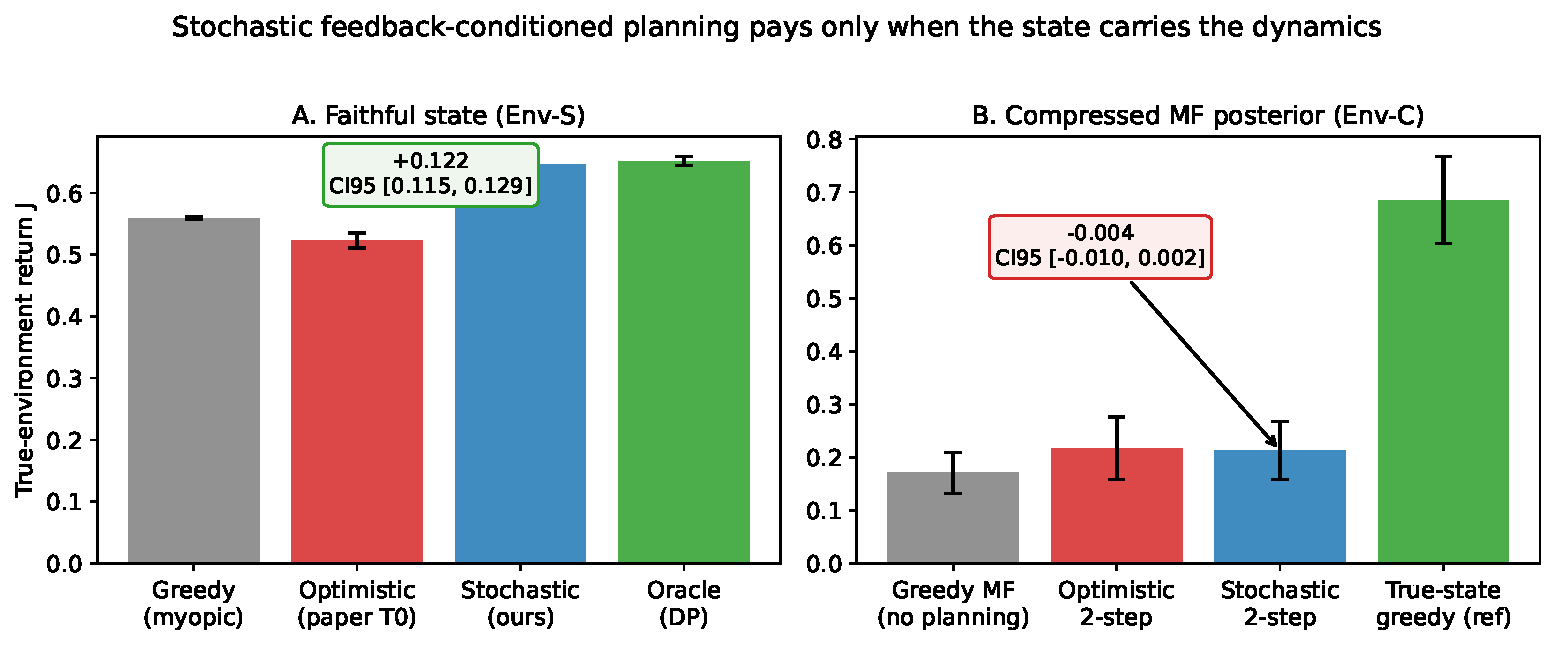
\includegraphics[width=\textwidth]{figures/main_figure.pdf}\\[2pt]
{\small\textbf{Рис.\,1.} Слева — честное состояние (Env-S); справа — сжатый MF-постериор (Env-C).}
\end{minipage}

\vspace{4pt}
\begin{center}
\colorbox{msgbg}{%
\begin{minipage}{0.96\textwidth}
\centering
\textbf{Ключевое сообщение:} стохастическое планирование окупается только когда представление
состояния несёт динамику: при честном состоянии оно достигает оракула ($+0.122$,
CI95 $[0.115, 0.129]$), над сжатым MF-постериором — не отличается от оптимистичного ($-0.004$).
\end{minipage}}
\end{center}

\vspace{2pt}
{\small
\noindent\textbf{Обозначения:} $J(\pi)$ — ожидаемая суммарная полезность политики $\pi$ в
истинной среде; T0 — оптимистичный переход; T1 — стохастическая модель отклика с точным
взвешенным обновлением; DP-оракул — точное решение методом обратной индукции.\quad
\textbf{Термины:} оптимистичный переход; feedback-conditioned transition; контролируемая
среда; сжатое состояние (MF-постериор).}

\vfill
\begin{center}
{\color{accent}\rule{\textwidth}{0.8pt}}\\[2pt]
{\small github.com/arinaromashkina/planning\_over\_MF\_MDP $\cdot$ \texttt{python run\_experiment.py} воспроизводит все числа и рисунки}
\end{center}

\end{document}
